% Author: Sebastian Sardina
\documentclass[a4paper,10pt]{standalone}
\usepackage{tikz}
\begin{document}
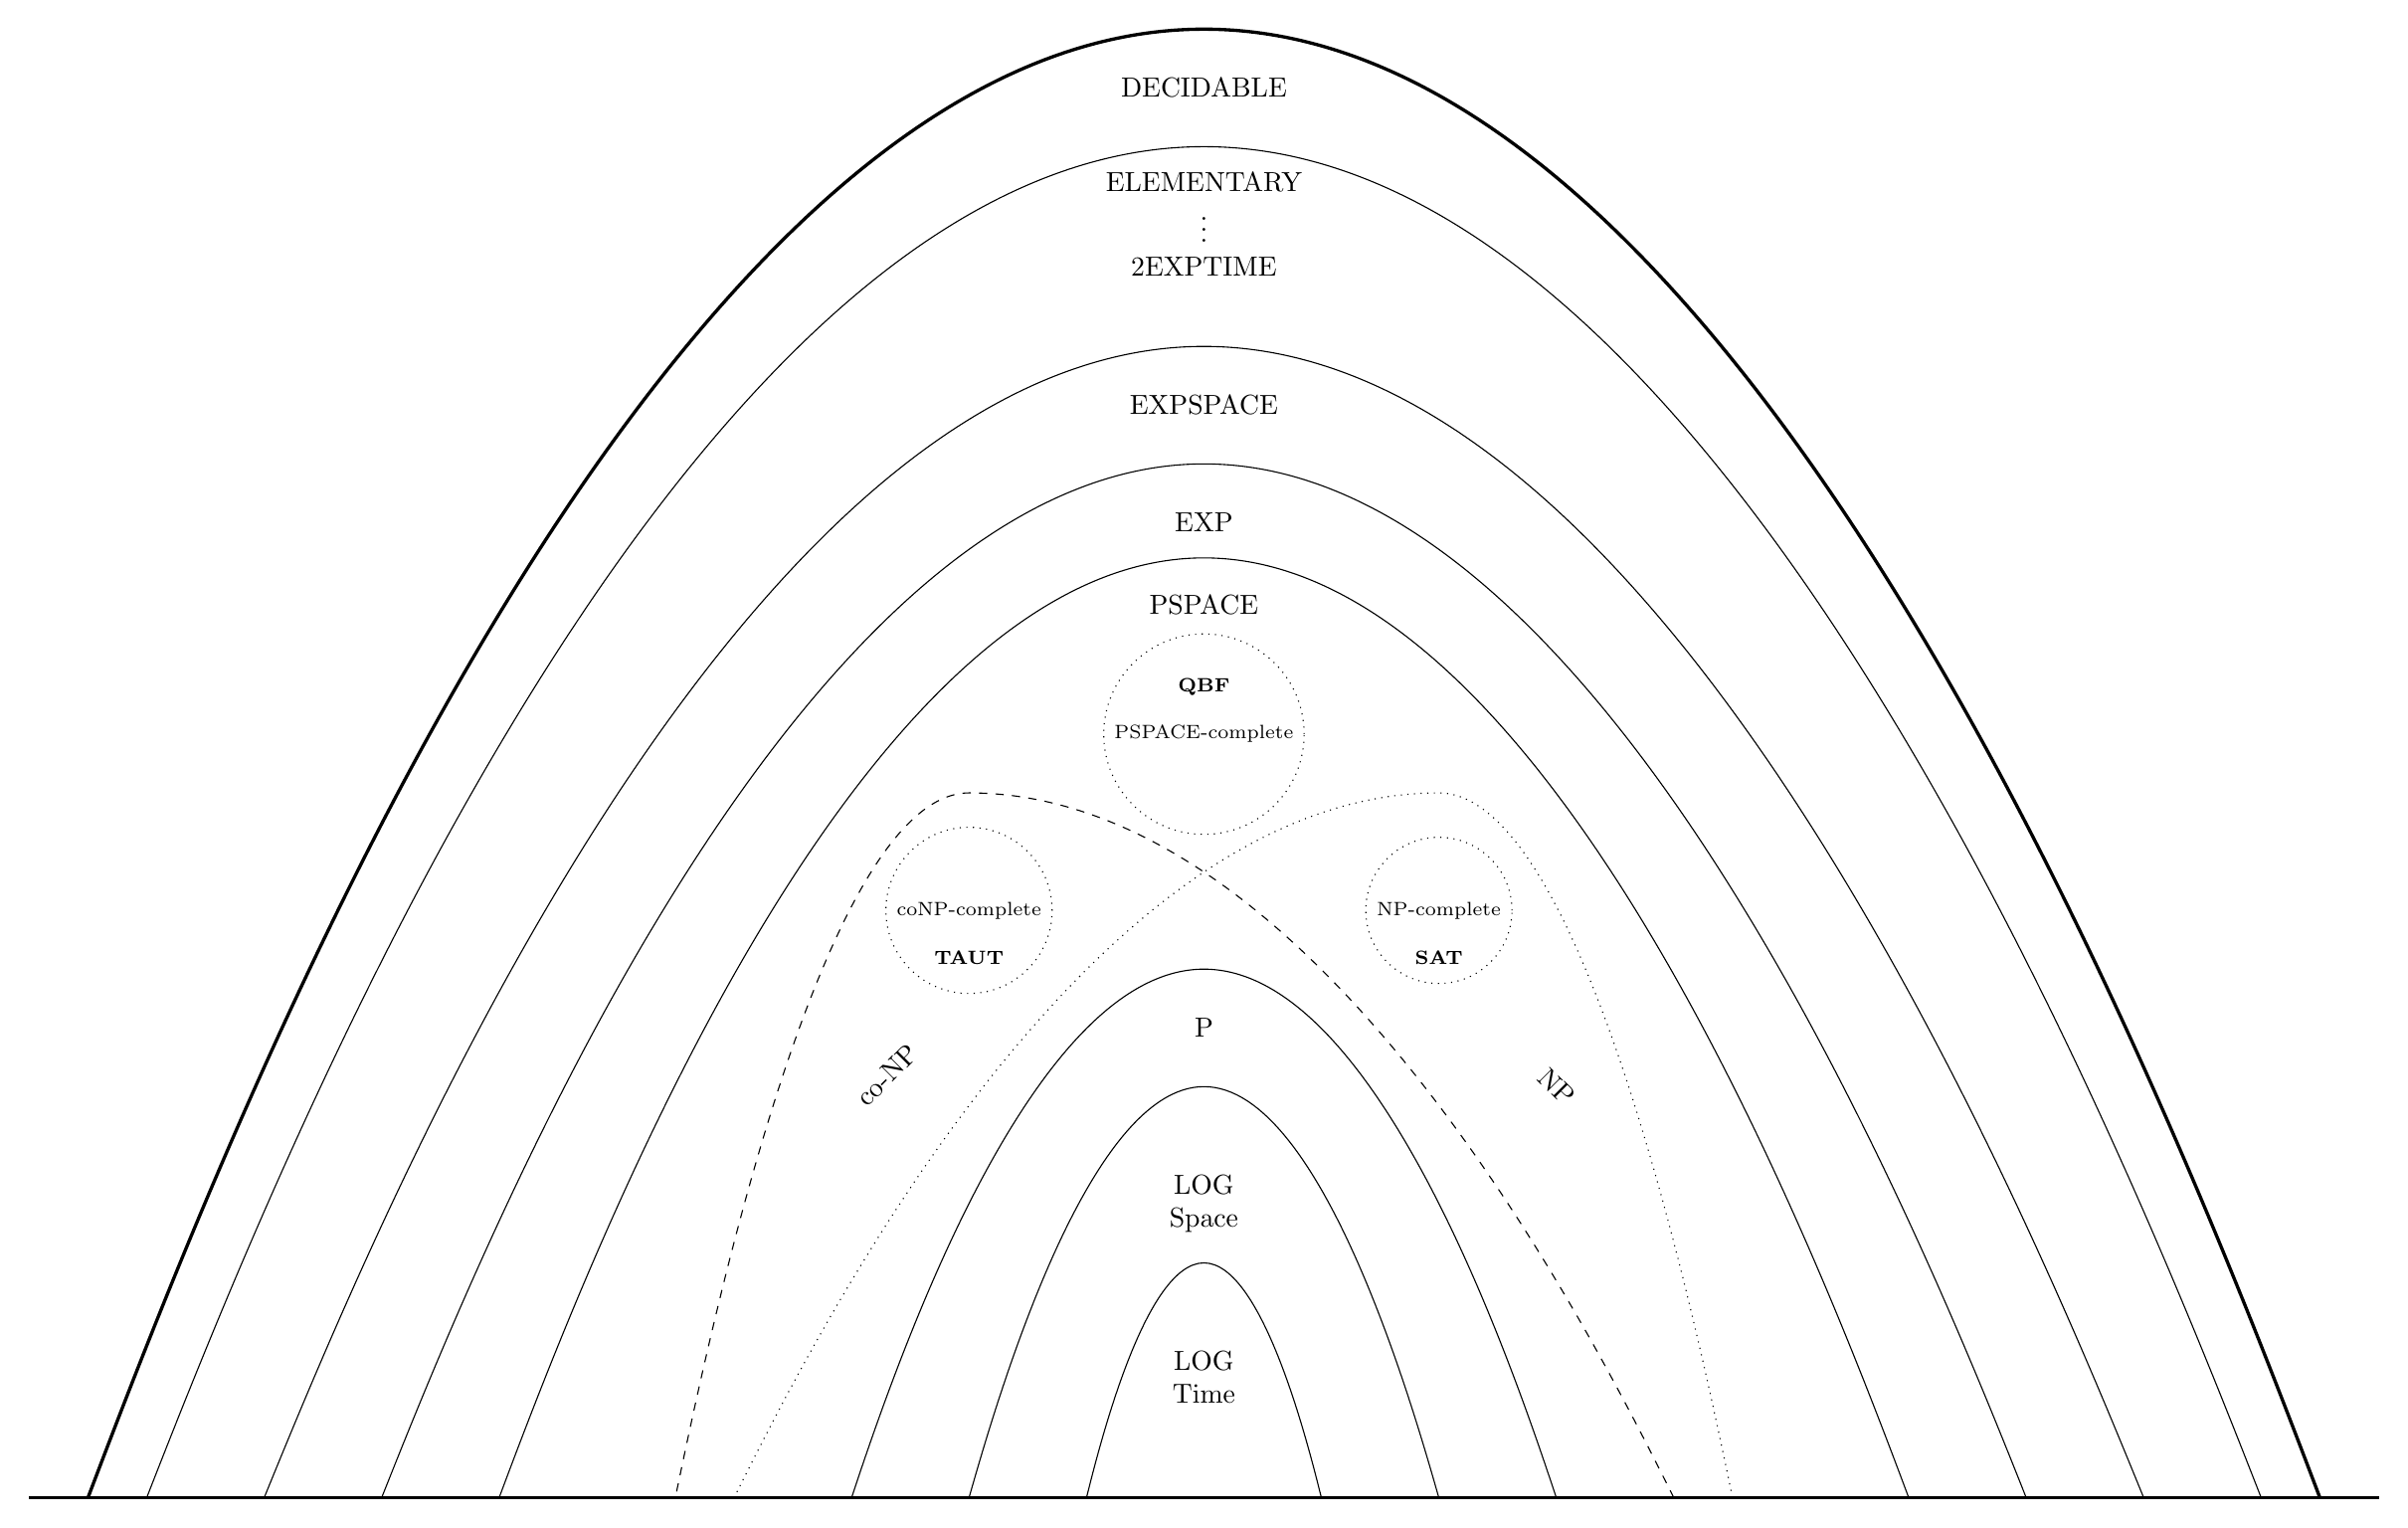
\begin{tikzpicture}
\pgftransformscale{1.5}

%%% HELP LINES - uncomment to design/extend
% \draw[step=1cm,gray,very thin] (-10,0) grid (10,12);
% \node at (0,0) {\textbf{(0,0)}};

%% Horizontal bar
\draw[very thick] (10,0) -- (-10,0);

% LOG TIME
\draw (-1,0) parabola bend (0,2) (1,0) ;
\node at (0,1) {
	\begin{tabular}{c}
	LOG \\ Time
	\end{tabular}
};

% LOG SPACE
\draw (-2,0) parabola bend (0,3.5) (2,0);
\node at (0,2.5) {
	\begin{tabular}{c}
	LOG \\ Space
	\end{tabular}
};

% PTIME
\draw (-3,0) parabola bend (0,4.5) (3,0);
\node at (0,4) {P};

% NP
\draw[dotted] (-4,0) parabola bend (2,6) (4.5,0);
\node[rotate=-45] at (3,3.5) {NP};

% NP-complete
\node[circle,dotted,draw] at (2,5) {\scriptsize NP-complete};

% SAT
\node[] at (2,4.6) {\scriptsize \textbf{SAT}};

% Co-NP
\draw[dashed] (4,0) parabola bend (-2,6) (-4.5,0);
\node[rotate=45] at (-2.7,3.6) {co-NP};

% Co-NP-complete
\node[circle,dotted,draw] at (-2,5) {\scriptsize coNP-complete};

% TAUT (i.e. validity problem)
\node[] at (-2,4.6) {\scriptsize \textbf{TAUT}};


% PSPACE
\draw (-6,0) parabola bend (0,8.0) (6,0);
\node at (0,7.6) {PSPACE};

% PSPACE-complete
\node[circle,dotted,draw] at (0,6.5) {\scriptsize PSPACE-complete};

% QBF
\node[] at (0,6.9) {\scriptsize \textbf{QBF}};

% EXPTIME
\draw (-7,0) parabola bend (0,8.8) (7,0);
\node at (0,8.3) {EXP};

% EXPSPACE
\draw (-8,0) parabola bend (0,9.8) (8,0);
\node at (0,9.3) {EXPSPACE};

% ELEMENTARY
\draw (-9,0) parabola bend (0,11.5) (9,0);
\node at (0,10.5) {};
\node[anchor=north] at (0,11.4) {
	\begin{tabular}{c}
		ELEMENTARY \\
		$\vdots$ \\
		2EXPTIME
	\end{tabular}
};

% RECURSIVE
\draw[very thick] (-9.5,0) parabola bend (0,12.5) (9.5,0);
\node at (0,12) {DECIDABLE};
\end{tikzpicture}
\end{document}